%!TEX root = uist14.tex
\section{Iteration 3: Head motion refinement}
\label{sec:iteration-3:-head}
\subsection{Problem Statement and Goal}
Both {\em Naive IR} and {\em Intensity IR} rely on list navigation on the
near-eye display for the refinement step. The list interface has a few clear shortcomings: navigation actions map poorly to real world results, and the users must switch their focus back and forth between the physical scene and the near-eye display. These problems motivated us to design an approach that harnesses the head orientation during the {\em refinement} stage.

In our third iteration, we build a system which further minimizes the chance of
falling back to list based {\em refinement}.

\subsection{Technique}
The motion sensors (including gyroscope, magnetometer and accelerometer) on the
head-worn device can help us determine the orientation of a user's head.
Unfortunately, this absolute orientation cannot be directly used in any indoor
environment as the user may change their location. As long as the targets are
spread around the periphery, however, their relative orientations are stable
(see Figure~\ref{fig:third_principle}). This key observation inspires us to
investigate a hybrid solution with IR and orientation sensors on Glass.

\begin{figure}[t]
\centering
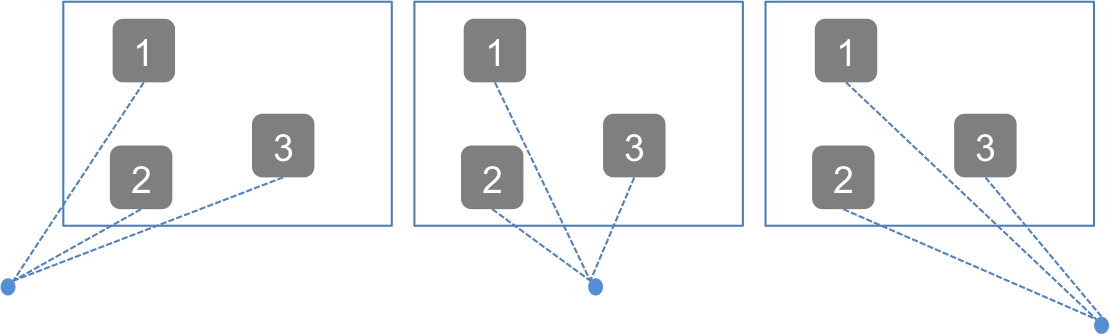
\includegraphics[width=1\columnwidth]{figures/third_principle.png}
\caption{Even when the user's absolution position changes, the relative relationship in the orientation space remain invariant.}
\label{fig:third_principle}
\end{figure}

\begin{figure}[t]
\centering
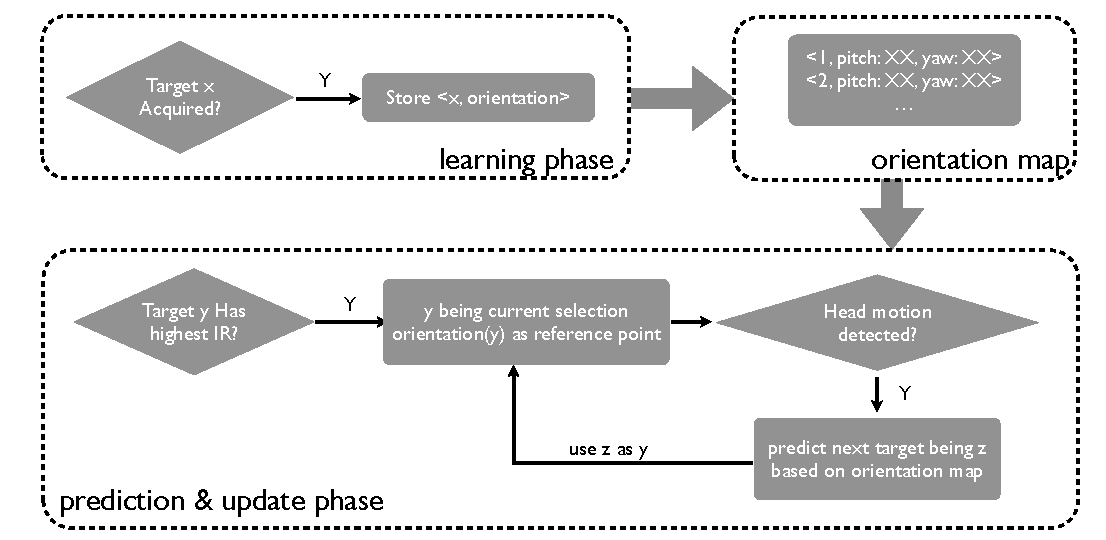
\includegraphics[width=1\columnwidth]{figures/third_technique3.pdf}
\caption{\ben{figure in interactionModel2.key file.} Our third technique learned each target's absolute orientation and construct the orientation map. Though we store the absolute orientation value, during the {\em refinement} stage, the prediction is only based on relative changes to a reference point. In such a way, the prediction will work regardless of user's position.}
\label{fig:third_technique}
\end{figure}

There are two phases to this technique: learning the relative orientations or
targets in a room and intelligently suggesting targets during refinement (see
Figure~\ref{fig:third_technique}).

In the first stage, the user orients their head towards each device, and the
system learns a map of the devices based on their corresponding sensor readings.
During the second stage, when the user wishes to use head-motion for
disambiguation, they will put their finger on the touchpad to enter a
quasi-mode, where only one device has a solid indicator light on at a time. This
gesture is inspired by observing users who tend to adjust their glasses for
closer inspection. The user can then tilt in the direction of the device they
wish to switch to. The system then uses its understanding of the relative
locations of the devices to create an {\em adjacency map}.

The technical implementation of this interaction involves a number of subtleties
due to the noisiness of our data. As mentioned earlier, absolute orientations
of devices change frequently at the slightest user movement. Unfortunately,
while relative orientation information is more stable, it does not contain
the necessary information for essential tasks, such as adding devices to a
learned map. To overcome these issues, we implement a hybrid method using
absolute and relative orientations augmented by IR information. Our system
stores the absolute orientations of each device during the learning stage, but
utilizes only the relative information for disambiguation. Once the user is in
quasi-mode, our system calculates the user's direction of motion using a
low-passed history of sensor measurements, and searches through the devices for
the nearest device in that direction. Thus, although the absolute orientations
may be incorrect, the relative information can still be used for disambiguation.

\subsection{Evaluation}
\ben{We then need evaluation results here, quantitative and qualitative.}
\bjoern{got to here in my pass}


% %!TEX root = uist14.tex
% \section{Iteration 3: Orientation-based refinement}
% \bjoern{While taking IR intensity into account further reduced the need for manual refinement and increased performance, the UI navigation scheme is problematic - it is not spatially related in any meaningful way to the layout of targets in a room. A better interaction technique would respect that ordering. For example, when refinement is needed, tilting the head slightly to the right could select the target that's adjacent to the right of the currently selected target.

% Such spatial navigation requires knowledge about the layout of targets in the environment. However, one of the strengths of our technique so far is that it does not require any map ahead of time. To enable some spatial navigation, we introduce a final iteration in which we build up a spatial data structure by demonstration (i.e., the user looks around the room) and then leverage that data structure during the refinement step of our interaction.}

% \bjoern{This technique is based on the assumption that users will generally select targets in indoor environments where targets are spread around the periphery. These assumptions enable us to use orientation data without knowing the user's absolute position.}

% \subsection{Implementation}
% \bjoern{give implementation details}

% \subsection{Informal User Feedback}
% \bjoern{We informally evaluate this technique with N users: ...}

 
%%% Local Variables: 
%%% mode: latex
%%% TeX-master: "uist14"
%%% End: 
